\chapter{Il sottolivello MAC e l'accesso multiplo}

% ══════════════════════════════════════════════════════════════
\section{I due tipi di collegamento}
% ══════════════════════════════════════════════════════════════

Ogni collegamento che abbiamo smontato finora aveva due estremi: un mittente, un ricevente, e nessun dubbio su a chi toccasse
parlare. Un \textbf{mezzo condiviso} cambia le cose: ciò che una stazione ci mette sopra è sentito da tutte le altre, e due che
trasmettono insieme si distruggono a vicenda. E non c'è un arbitro: nessun master, nessun canale separato su cui chiedere il
permesso. Le regole vanno concordate \textbf{sullo stesso canale per cui si compete}.

È il \textbf{problema dell'accesso multiplo}, e il sottolivello \textbf{MAC} è la parte del livello di collegamento che lo risolve. Fra
i quattro servizi del livello di collegamento è il secondo, l'\textbf{accesso al collegamento}. Vedremo tre famiglie di regole, per
ciascuna che cosa compra e che cosa costa, e poi l'argomento sui tempi che ha dato forma a Ethernet.

I collegamenti da gestire sono essenzialmente di due tipi.

\dfn{Collegamento punto-punto e broadcast}{
    \begin{itemize}
      \item Un collegamento \textbf{punto-punto} ha un solo mittente a un'estremità e un solo ricevente all'altra. Un protocollo che
            gestisce collegamenti di questo tipo è il \textbf{PPP} (\emph{Point-to-Point Protocol}). Esempio: un cavo Ethernet diretto
            tra due computer.
      \item Un collegamento \textbf{broadcast} ha più nodi mittenti e riceventi collegati allo \textbf{stesso canale condiviso}. Si
            chiama broadcast perché quando un nodo trasmette un frame, questo viene \textbf{ricevuto da tutti} i nodi sul canale.
            Esempi: il bus Ethernet, Ethernet half-duplex (raro, oggi i cavi sono quasi tutti full-duplex), le LAN wireless.
    \end{itemize}
}

\begin{figure}[H]
\centering
\begin{tikzpicture}[every node/.style={font=\footnotesize\sffamily}]
  \begin{scope}
    \node[font=\small\bfseries\sffamily] at (2,1.6) {Punto-punto};
    \node (a) at (0,0) {\icon[1cm]{pc}}; \node[below=-2pt of a] {invia A};
    \node (b) at (4,0) {\icon[1cm]{laptop}}; \node[below=-2pt of b, text=netgreen!60!black] {accetta A};
    \draw[wired, line width=1.6pt] (a) -- node[above] {PPP} (b);
  \end{scope}
  \begin{scope}[xshift=7.5cm]
    \node[font=\small\bfseries\sffamily] at (2.5,1.6) {Broadcast};
    \draw[backbone] (-0.2,0) -- (5.2,0);
    \foreach \x/\ic/\t/\c in {0/pc/{invia A}/black, 1.7/laptop/{scarta A}/netred, 3.4/pc/{accetta A}/netgreen!60!black, 5/laptop/{scarta A}/netred} {
      \node (n) at (\x,0.8) {\icon[0.7cm]{\ic}}; \draw[wired] (\x,0) -- (n);
      \node[text=\c] at (\x,-0.4) {\t};
    }
  \end{scope}
\end{tikzpicture}
\caption{Nel broadcast tutti ricevono il frame, e solo il destinatario lo accetta.}
\end{figure}

L'accesso ai collegamenti broadcast va \textbf{coordinato} (\emph{problema dell'accesso multiplo}), perché più comunicazioni sullo
stesso collegamento possono interferire tra loro.

% ══════════════════════════════════════════════════════════════
\section{Le collisioni}
% ══════════════════════════════════════════════════════════════

\dfn{Collisione}{
    Il problema principale dei collegamenti broadcast è la \textbf{collisione}: se più nodi trasmettono frame \textbf{contemporaneamente}
    sullo stesso canale, i frame si sovrappongono e diventano \textbf{incomprensibili}.
}

I segnali si sommano sul mezzo e nessun ricevente riesce a dare un senso a nessuno dei due frame. I frame rovinati arrivano a
tutti e falliscono il controllo (il CRC del capitolo precedente), quindi vengono scartati come errati. I costi sono due:

\begin{itemize}
    \item \textbf{tutti} i frame coinvolti vanno \textbf{persi}, e ogni mittente deve riprovare;
    \item l'intervallo di tempo è \textbf{sprecato}: il canale è stato occupato per tutto il tempo e non ha portato nulla.
\end{itemize}

\begin{figure}[H]
\centering
\begin{tikzpicture}[every node/.style={font=\footnotesize\sffamily}]
  \draw[backbone] (-0.2,0) -- (8.2,0);
  \node (a) at (0,0.8) {\icon[0.7cm]{pc}}; \draw[wired] (0,0) -- (a); \node[above=-1pt of a] {invia A};
  \node (b) at (8,0.8) {\icon[0.7cm]{pc}}; \draw[wired] (8,0) -- (b); \node[above=-1pt of b] {invia B};
  \node (c) at (2.7,0.8) {\icon[0.8cm]{laptop}}; \draw[wired] (2.7,0) -- (c); \node[above=-1pt of c, text=netred] {scarta \$@!};
  \node (d) at (5.3,0.8) {\icon[0.8cm]{laptop}}; \draw[wired] (5.3,0) -- (d); \node[above=-1pt of d, text=netred] {scarta \$@!};
  \draw[-{Stealth}, very thick, netblue] (0.3,-0.3) -- (4.8,-0.3);
  \draw[-{Stealth}, very thick, netorange] (7.7,-0.45) -- (3.2,-0.45);
  \node[starburst, draw=netred, fill=netred!20, minimum size=0.9cm, inner sep=0pt, font=\scriptsize\bfseries\sffamily] at (4,-0.9) {collisione!};
\end{tikzpicture}
\caption{Due trasmissioni contemporanee sullo stesso canale collidono: tutti i nodi ricevono dati illeggibili.}
\end{figure}

L'accesso al mezzo fisico (come il framing) è regolato dal protocollo \textbf{MAC} (\emph{Medium Access Control}), un
\textbf{sottolivello} del livello di collegamento.

% ══════════════════════════════════════════════════════════════
\section{I protocolli ad accesso multiplo}
% ══════════════════════════════════════════════════════════════

Nelle reti i \textbf{protocolli ad accesso multiplo} regolano le trasmissioni sui canali broadcast in modo che:

\begin{itemize}
    \item le collisioni siano \textbf{gestite};
    \item ogni nodo abbia la possibilità di trasmettere, e nessuno \textbf{monopolizzi} il collegamento;
    \item le connessioni già stabilite non vengano interrotte (per esempio controllando se il collegamento è occupato).
\end{itemize}

Servono in molti contesti, dove centinaia o migliaia di nodi possono stare su un unico canale broadcast:

\begin{itemize}
    \item \textbf{filo condiviso}: il cavo coassiale di una rete di accesso via cavo, con la centrale (\emph{head end}) a un capo e le
          case lungo il cavo;
    \item \textbf{senza fili condiviso}: ogni stazione nel raggio di un access point trasmette nella stessa aria;
    \item \textbf{satellite}: stazioni a terra a migliaia di chilometri l'una dall'altra, tutte ascoltate dallo stesso transponder.
\end{itemize}

Tecnologie diverse, un solo problema. Ne esistono decine di soluzioni; gli approcci principali sono tre:

\begin{itemize}
    \item \textbf{partizionamento del canale}: la capacità viene divisa \textbf{in anticipo} e ogni nodo riceve un pezzo, una volta per
          tutte;
    \item \textbf{accesso casuale}: nessuno riceve nulla; un nodo trasmette a piena velocità, collide, e riprova;
    \item \textbf{a turni} (\emph{taking turns}): il diritto di trasmettere viene passato di mano, così che un solo nodo alla volta ne
          abbia titolo.
\end{itemize}

Differiscono per \textbf{quando} avviene l'arbitraggio: prima della trasmissione, dopo, o attorno ad essa. Ogni protocollo reale
appartiene a una delle tre famiglie, oppure (come vedremo alla fine) le usa tutte e tre in parti diverse della stessa rete.

\dfn{Le proprietà desiderate}{
    Un protocollo ad accesso multiplo per un canale broadcast a $R$ bit/s dovrebbe avere quattro proprietà:
    \begin{enumerate}
      \item se un solo nodo deve trasmettere, quel nodo ottiene \textbf{tutto $R$}: il canale non è rallentato dalle stazioni assenti;
      \item se $M$ nodi devono trasmettere, ciascuno ottiene \textbf{in media $R/M$}, non istante per istante ma su un intervallo
            ragionevole;
      \item \textbf{decentralizzato}: nessun nodo master, perché un master è un single point of failure per tutto il canale;
      \item \textbf{semplice ed economico}: le regole girano su ogni frame, in hardware, quindi ogni overhead si paga milioni di volte.
    \end{enumerate}
    Nessun protocollo le ha tutte e quattro, e \textbf{quale sacrifica} è ciò che distingue una famiglia dall'altra.
}

\dfn{Il modello dietro ogni protocollo}{
    \begin{itemize}
      \item \textbf{Un canale}: $N$ stazioni, tutte trasmettono e ricevono su di esso, e non c'è un canale laterale su cui negoziare.
      \item \textbf{Collisioni osservabili}: i frame sovrapposti si rovinano e vanno persi, e una stazione può accorgersi che è
            successo.
      \item \textbf{Tempo continuo o a slot}: gli slot richiedono un orologio su cui tutte le stazioni siano d'accordo, e non ogni
            collegamento può fornirlo.
      \item \textbf{Ascolto della portante, o no}: se una stazione può capire che il canale è occupato prima di cominciare.
    \end{itemize}
    I protocolli che seguono differiscono soprattutto nel modo in cui rispondono alle ultime due.
}

% ══════════════════════════════════════════════════════════════
\section{Protocolli a partizionamento del canale}
% ══════════════════════════════════════════════════════════════

\subsection{TDMA}

\dfn{TDMA (Time Division Multiple Access)}{
    Dato un canale con $N$ nodi e velocità $R$ bit/s, il \textbf{TDMA} divide il tempo in \textbf{trame} (\emph{frame} temporali) e ogni
    trama in $N$ \textbf{slot}. Ogni slot è assegnato a uno degli $N$ nodi: quando un nodo ha un pacchetto da inviare, aspetta il proprio
    slot. Di solito la dimensione degli slot è scelta in modo che un pacchetto intero possa essere trasmesso in uno slot. Niente
    collisioni, ed equità perfetta: ognuno ottiene $R/N$ in ogni trama.
}

\warning{Attenzione alla parola}{
    Una \emph{trama} (\emph{frame}) di TDM non è un frame di collegamento: qui è un giro dell'orologio, che contiene uno slot per
    ciascun nodo.
}

\subsection{FDMA}

\dfn{FDMA (Frequency Division Multiple Access)}{
    Il \textbf{FDMA} divide il canale da $R$ bit/s in \textbf{frequenze diverse}, ciascuna con banda $R/N$, e assegna ogni frequenza a uno
    degli $N$ nodi. Tutti i nodi trasmettono contemporaneamente e in permanenza, ciascuno nella propria banda: il canale è tagliato
    in frequenza, non a turni.
}

\begin{figure}[H]
\centering
\begin{tikzpicture}[every node/.style={font=\scriptsize\sffamily}]
  \begin{scope}
    \node[font=\footnotesize\bfseries\sffamily] at (2.8,2.6) {TDMA};
    \draw[-{Stealth}] (0,0) -- (6,0) node[right] {tempo}; \draw[-{Stealth}] (0,0) -- (0,2.3) node[above] {frequenza};
    \foreach \k in {0,1} \foreach \i/\c in {1/lapp,2/ltra,3/lnet,4/llink} { \fill[\c] (0.1+\k*2.8+\i*0.65-0.65,0.1) rectangle ++(0.6,1.9); \node at (0.4+\k*2.8+\i*0.65-0.65,1.05) {N\i}; }
    \draw[decorate, decoration={brace, amplitude=4pt, mirror}] (0.1,-0.15) -- (2.7,-0.15) node[midway, below=4pt] {trama};
    \draw[decorate, decoration={brace, amplitude=3pt}] (0.1,2.05) -- (0.7,2.05) node[midway, above=3pt] {slot};
  \end{scope}
  \begin{scope}[xshift=7.8cm]
    \node[font=\footnotesize\bfseries\sffamily] at (2.8,2.6) {FDMA};
    \draw[-{Stealth}] (0,0) -- (6,0) node[right] {tempo}; \draw[-{Stealth}] (0,0) -- (0,2.3) node[above] {frequenza};
    \foreach \i/\c in {1/lapp,2/ltra,3/lnet,4/llink} { \fill[\c] (0.1,0.1+\i*0.48-0.48) rectangle ++(5.6,0.44); \node at (2.9,0.32+\i*0.48-0.48) {N\i}; }
  \end{scope}
\end{tikzpicture}
\caption{TDMA: a turno, ciascuno con tutta la banda. FDMA: sempre, ciascuno con una fetta della banda.}
\end{figure}

FDMA e TDMA condividono pro e contro:

\begin{itemize}
    \item[\itick] \textbf{evitano le collisioni} e dividono la banda \textbf{equamente} tra gli $N$ nodi;
    \item[\icross] un nodo è limitato a una banda di $R/N$ \textbf{anche quando è l'unico} ad avere pacchetti da inviare: capacità sprecata.
\end{itemize}

\subsection{Quanto costa una divisione fissa}

L'argomento l'abbiamo già incontrato confrontando circuiti e pacchetti: la capacità riservata è sprecata ogni volta che il suo
proprietario tace. Qui si può misurare. Su un canale di capacità $C$ bit/s, con frame che arrivano a un tasso di $\lambda$ frame al
secondo e lunghezza media $1/\mu$ bit, il ritardo medio (teoria delle code) è
$$T = \frac{1}{\mu C - \lambda}.$$
Dividiamo lo stesso canale in $N$ sottocanali da $C/N$, ciascuno dei quali riceve $\lambda/N$ frame al secondo:
$$T_N = \frac{1}{\mu (C/N) - \lambda/N} = \frac{N}{\mu C - \lambda} = N\,T.$$

\begin{esempio}{Una coda per tutte le casse, o una coda ciascuna}
$C = 100$ Mb/s, frame lunghi in media $1/\mu = 10\,000$ bit, $\lambda = 5000$ frame/s. Il canale smaltisce $\mu C = 10\,000$ frame/s,
quindi $T = 1/(10\,000 - 5000)\ \text{s} = 200\ \mu\text{s}$. Diviso in 10 sottocanali, il ritardo medio diventa $T_{10} = 2$ ms.
\end{esempio}

Il partizionamento \textbf{moltiplica il ritardo medio per $N$}: è la differenza tra un'unica fila per tutte le casse e una fila per
ciascuna. Va bene dove il carico è costante e noto; è sbagliato dove è a raffiche, e il traffico dei calcolatori è a raffiche.

\subsection{CDMA}

\dfn{CDMA (Code Division Multiple Access)}{
    Il \textbf{CDMA} assegna a ogni nodo un \textbf{codice} diverso, con cui codifica e decodifica i bit che invia. Se i codici sono scelti con
    cura, nelle reti CDMA più nodi possono trasmettere \textbf{contemporaneamente, sulle stesse frequenze}, senza interferire.
}

\begin{esempio}{L'idea del CDMA}
Siano $c_A = (+1, -1)$ e $c_B = (+1, +1)$ i codici di due stazioni: sono \textbf{ortogonali}, cioè il loro prodotto scalare è
$c_A \cdot c_B = 1 - 1 = 0$, mentre $c_B \cdot c_B = 2$. Per trasmettere un bit, ogni stazione invia il proprio codice moltiplicato per
$+1$ (bit 1) o $-1$ (bit 0). Sul canale i segnali si \textbf{sommano}.
\begin{itemize}
    \item A invia 1, B invia 1: sul canale arriva $c_A + c_B = (2, 0)$.
    \item Il ricevente di B calcola $(c_A + c_B)\cdot c_B = c_A\cdot c_B + c_B \cdot c_B = 0 + 2 > 0$: B ha inviato \textbf{1}.
    \item Il ricevente di A calcola $(c_A + c_B)\cdot c_A = 2 + 0 > 0$: anche A ha inviato \textbf{1}.
\end{itemize}
Il contributo dell'altra stazione si annulla grazie all'ortogonalità dei codici. Normalizzando il prodotto scalare (dividendo per la
lunghezza del codice) il prodotto di un codice con sé stesso vale 1, e la relazione si scrive
$$(c_A + c_B)\cdot c_B = \underbrace{c_A\cdot c_B}_{=0} + \underbrace{c_B\cdot c_B}_{=1} = 1:$$
il bit di B sopravvive e quello di A sparisce, anche se le due stazioni hanno trasmesso insieme. La collisione \textbf{non avviene affatto}.
\end{esempio}

\begin{itemize}
    \item Né tempo né frequenza: tutti i nodi trasmettono insieme, su tutta la banda, sempre, e i riceventi li separano comunque.
    \item Si usa dove il mezzo non si può tagliare in modo pulito, soprattutto sui canali \textbf{senza fili}: da tempo in ambito
          militare (per la resistenza ai disturbi intenzionali, il \emph{jamming}) e nella telefonia cellulare (per esempio il 3G).
    \item[\icross] È complesso da realizzare.
    \item[\icross] Non scala bene con il numero di nodi.
\end{itemize}

\info{Il segnale modulato}{
    Sui canali radio i dati non viaggiano ``così come sono'': si trasmette un segnale in \textbf{banda base} (a bassa frequenza) modulando una
    \textbf{frequenza portante} più alta. Il telefono analogico, per esempio, usa la banda 300--3400 Hz. FDMA e CDMA lavorano proprio sulle
    frequenze portanti e sulla loro condivisione.
}

% ══════════════════════════════════════════════════════════════
\section{Protocolli ad accesso casuale}
% ══════════════════════════════════════════════════════════════

\dfn{Accesso casuale}{
    Nei protocolli ad \textbf{accesso casuale} un nodo che trasmette usa sempre \textbf{tutta la velocità} del canale ($R$ bit/s). Se avviene
    una collisione (almeno due nodi trasmettono insieme), ogni nodo coinvolto \textbf{aspetta un ritardo casuale} prima di ritrasmettere.
}

Le collisioni non vengono \textbf{prevenute}, vengono \textbf{riparate}. Il ritardo deve essere casuale ed estratto
\textbf{indipendentemente}: due stazioni che aspettassero lo stesso tempo fisso collidirebbero per sempre. Se le due estrazioni sono
abbastanza diverse, uno dei due nodi riesce a ``infilare'' il proprio frame; se non lo sono, avviene una nuova collisione e una nuova
estrazione. Tutta la famiglia vive di questa scommessa, e ciò che segue è una serie di modi per migliorare le probabilità.

\subsection{ALOHA puro}

Il primo protocollo ad accesso casuale nacque alle Hawaii nel 1970 (ALOHAnet): terminali sparsi su diverse isole, nessun cavo che
valesse la pena di posare, e una stazione centrale a Honolulu.

\begin{itemize}
    \item La regola: ogni stazione trasmette \textbf{appena ha un frame} da inviare. Il protocollo non ha altro.
    \item La stazione centrale ritrasmette ogni frame che riceve: una stazione che sente tornare indietro il proprio frame sa che è
          arrivato. Il riscontro è l'\textbf{eco}, e non costa nulla in più.
    \item Il silenzio significa collisione: si attende un tempo casuale e si ritrasmette.
\end{itemize}

\begin{figure}[H]
\centering
\begin{tikzpicture}[every node/.style={font=\scriptsize\sffamily}]
  \foreach \y/\n in {0/A, -0.7/B, -1.4/C} { \node[anchor=east] at (-0.2,\y) {\n}; \draw[black!30] (0,\y) -- (11,\y); }
  \draw[-{Stealth}] (0,-1.9) -- (11,-1.9) node[right] {tempo};
  \fill[netblue!40] (0.5,-0.2) rectangle (2.5,0.2);
  \fill[netred!40] (2.0,-0.9) rectangle (4.0,-0.5); \fill[netred!40] (3.4,-1.6) rectangle (5.4,-1.2);
  \fill[netblue!40] (5.8,-0.2) rectangle (7.8,0.2); \fill[netblue!40] (8.4,-0.9) rectangle (10.4,-0.5);
  \draw[netred, very thick] (2.0,-1.05) -- (5.4,-1.05);
  \node[text=netred] at (3.7,-2.25) {B e C si sovrappongono (e B anche con A): collisioni};
  \draw[dashed] (2,0.4) -- (2,-1.9); \draw[dashed] (2.5,0.4) -- (2.5,-1.9);
\end{tikzpicture}
\caption{ALOHA puro: basta che due frame si sovrappongano anche in parte perché entrambi vadano persi.}
\end{figure}

\subsubsection*{Il periodo di vulnerabilità}

Sia $t$ il tempo per trasmettere un frame. Il frame in esame sopravvive solo se \textbf{nessun altro comincia} in una finestra di
$2t$ attorno ad esso: tutto ciò che è iniziato nel tempo di frame precedente ne colpisce l'inizio, tutto ciò che inizia durante ne
colpisce la fine. E basta un solo bit sovrapposto: il controllo scarta il frame comunque, e uno sfioramento costa quanto un urto
frontale.

\begin{figure}[H]
\centering
\begin{tikzpicture}[every node/.style={font=\scriptsize\sffamily}]
  \draw[-{Stealth}] (0.5,0) -- (10,0) node[right] {tempo};
  \foreach \x/\l in {2/{$t_0$}, 4.5/{$t_0+t$}, 7/{$t_0+2t$}} \draw (\x,0.08) -- (\x,-0.08) node[below] {\l};
  \foreach \x in {2,7} \draw[dashed, black!40] (\x,0) -- (\x,2.1);
  \fill[netblue!40] (4.5,0.25) rectangle (7,0.85); \node at (5.75,0.55) {frame in esame};
  \fill[netred!30] (2.6,1.15) rectangle (5.1,1.75); \node at (3.85,1.45) {ne colpisce l'inizio};
  \fill[netred!30] (6.3,1.15) rectangle (8.8,1.75); \node at (7.55,1.45) {ne colpisce la fine};
  \draw[decorate, decoration={brace, amplitude=5pt, mirror}] (2,-0.5) -- (7,-0.5) node[midway, below=6pt, text=netred] {periodo vulnerabile: due tempi di frame};
\end{tikzpicture}
\caption{In ALOHA puro un frame è vulnerabile per $2t$: qualunque altro frame iniziato in quella finestra lo distrugge.}
\end{figure}

\subsubsection*{Al massimo il diciotto per cento}

Sia $G$ il numero di tentativi di trasmissione per tempo di frame, frame nuovi e ritrasmissioni insieme, e supponiamo che arrivino a
caso (secondo Poisson). La finestra vulnerabile è lunga due tempi di frame, quindi la probabilità che nessun altro inizi in essa è
$e^{-2G}$, e il throughput (frame riusciti per tempo di frame) è
$$S = G\,e^{-2G}.$$
Il massimo è a $G = 0{,}5$, dove $S = 1/2e \approx 0{,}18$: con tutti che trasmettono a piacere, il \textbf{18\%} del canale. Oltre il
picco, offrire più carico dà \textbf{meno} throughput: il canale crolla sotto le proprie ritrasmissioni. È il prezzo del non assumere
nulla: niente orologio, niente ascolto, nessun coordinamento.

\subsection{Slotted ALOHA}

\dfn{Slotted ALOHA}{
    \begin{itemize}
      \item Il tempo è diviso in \textbf{slot} di $L/R$ secondi (esattamente un frame di $L$ bit), come in TDMA.
      \item I nodi sono \textbf{sincronizzati}: ogni nodo trasmette frame solo \textbf{all'inizio} di uno slot.
      \item Se nello slot non c'è collisione, la comunicazione prosegue; se c'è, tutte le stazioni coinvolte se ne accorgono
            prima che lo slot finisca.
      \item Se c'è una collisione, ogni nodo coinvolto ritrasmette il frame in ciascuno degli slot successivi \textbf{con probabilità
            $p \in [0,1]$} (``lancia una moneta''), finché il frame non viene inviato con successo.
    \end{itemize}
}

\begin{figure}[H]
\centering
\begin{tikzpicture}[every node/.style={font=\scriptsize\sffamily}]
  \foreach \x in {0,1.5,...,9} \draw[dashed, black!30] (\x,0.6) -- (\x,-1.6);
  \node[anchor=east] at (-0.2,0) {nodo 1}; \node[anchor=east] at (-0.2,-1) {nodo 2};
  \draw[-{Stealth}] (0,-1.6) -- (9.3,-1.6) node[right] {tempo};
  \fill[netred!40] (0,-0.2) rectangle (1.5,0.2); \fill[netred!40] (0,-1.2) rectangle (1.5,-0.8);
  \node[text=netred] at (0.75,-0.5) {collisione};
  \node at (2.25,0) {non invia}; \node at (2.25,-1) {non invia};
  \fill[netred!40] (3,-0.2) rectangle (4.5,0.2); \fill[netred!40] (3,-1.2) rectangle (4.5,-0.8);
  \node[text=netred] at (3.75,-0.5) {collisione};
  \fill[netgreen!40] (4.5,-0.2) rectangle (6,0.2); \node at (5.25,0) {invia};
  \node at (5.25,-1) {non invia};
  \fill[netgreen!40] (7.5,-1.2) rectangle (9,-0.8); \node at (8.25,-1) {invia};
  \node[text=netgreen!50!black] at (5.25,0.45) {successo}; \node[text=netgreen!50!black] at (8.25,-0.55) {successo};
\end{tikzpicture}
\caption{Slotted ALOHA: dopo una collisione, in ogni slot ciascun nodo ritrasmette con probabilità $p$.}
\end{figure}

Le monete sono \textbf{indipendenti}, ed è l'unica ragione per cui le due stazioni prima o poi si separano.

\begin{itemize}
    \item[\itick] Se c'è un solo nodo, usa tutta la velocità $R$ del canale (niente collisioni).
    \item[\itick] È \textbf{decentralizzato}: i nodi sono del tutto indipendenti tra loro, a parte la sincronizzazione.
    \item[\itick] È \textbf{semplice} da realizzare ed eseguire (la scelta casuale è velocissima).
    \item[\itick] Più collisioni consecutive sono improbabili.
\end{itemize}

Ora nulla può sovrapporsi \textbf{in parte} a un frame, quindi la finestra vulnerabile si riduce da due tempi di frame a uno, e
$$S = G\,e^{-G}.$$
Il picco si sposta a $G = 1$ e sale a $1/e \approx 0{,}37$: esattamente il \textbf{doppio} dell'ALOHA puro. Al picco il 37\% degli
slot va a buon fine, il 37\% resta vuoto e il 26\% contiene collisioni: un canale da 100 Mb/s che ne fa 37.

\begin{figure}[H]
\centering
\begin{tikzpicture}
  \begin{axis}[width=10cm, height=5cm, xlabel={$G$ (tentativi per slot, cioè per tempo di frame)}, ylabel={$S$ (throughput per frame)},
      xmin=0, xmax=3, ymin=0, ymax=0.42, grid=major, grid style={gray!20}, legend pos=north east,
      legend style={font=\scriptsize\sffamily}, tick label style={font=\scriptsize}, label style={font=\footnotesize\sffamily}]
    \addplot[very thick, netblue, domain=0:3, samples=80] {x*exp(-x)}; \addlegendentry{slotted ALOHA: $S = Ge^{-G}$}
    \addplot[very thick, netred, domain=0:3, samples=80] {x*exp(-2*x)}; \addlegendentry{ALOHA puro: $S = Ge^{-2G}$}
    \addplot[only marks, mark=*, netblue] coordinates {(1,0.368)}; \addplot[only marks, mark=*, netred] coordinates {(0.5,0.184)};
  \end{axis}
\end{tikzpicture}
\caption{Throughput di ALOHA: al meglio lo slotted ALOHA usa il canale per il 37\% del tempo ($1/e$), l'ALOHA puro solo il 18\% ($1/2e$).}
\end{figure}

\warning{Che cosa gli slot non risolvono}{
    Due stazioni decidono di trasmettere a metà dello stesso slot. Che succede? Entrambe aspettano il confine successivo, entrambe
    partono lì, ed entrambi i frame vanno distrutti: gli slot \textbf{non eliminano le collisioni}. Eliminano la sovrapposizione
    \textbf{parziale}: un frame non può più essere rovinato da uno iniziato un attimo prima, e le trasmissioni sono ora o
    perfettamente allineate o del tutto disgiunte. Dimezzare la finestra vulnerabile è tutto il guadagno, e il prezzo è un
    \textbf{orologio comune} a tutte le stazioni: su un collegamento lungo, o radio, non è gratis.
}

\subsection{CSMA e CSMA/CD}

Entrambi gli ALOHA trasmettono \textbf{alla cieca}: una stazione decide senza alcun riguardo per ciò che c'è sul canale in quel
momento, e si può cominciare a trasmettere (producendo una collisione) anche se il canale \textbf{è già occupato}. La soluzione sono le
regole della conversazione educata: \textbf{ascoltare prima di parlare}, e smettere se si parla sopra qualcuno.

\dfn{CSMA e CSMA/CD}{
    I protocolli \textbf{CSMA} (\emph{Carrier Sense Multiple Access}) e \textbf{CSMA/CD} (CSMA con \emph{Collision Detection}) si basano su
    due principi:
    \begin{itemize}
      \item \textbf{carrier sensing}: i nodi ascoltano il canale \textbf{prima} di trasmettere. Se un altro nodo sta trasmettendo un frame,
            aspettano che la trasmissione finisca;
      \item \textbf{collision detection}: i nodi ascoltano il canale \textbf{mentre} trasmettono. Se rilevano una collisione, smettono di
            trasmettere e aspettano un tempo casuale prima di riprovare.
    \end{itemize}
}

Ma se tutti i nodi ascoltano prima di trasmettere, perché avvengono comunque collisioni? Per il \textbf{ritardo di propagazione} del
segnale.

\begin{figure}[H]
\centering
\begin{minipage}{0.34\linewidth}\centering
  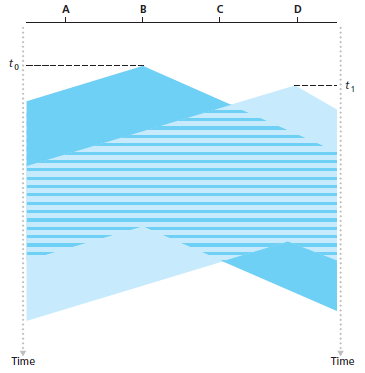
\includegraphics[width=0.9\linewidth]{cap19/csma_ritardo.png}
\end{minipage}\hfill
\begin{minipage}{0.62\linewidth}
\begin{itemize}
  \item Anche se la propagazione è vicina alla velocità della luce, il segnale impiega del \textbf{tempo} per raggiungere gli altri nodi.
  \item Nella figura (spazio in orizzontale, tempo verso il basso) B comincia a trasmettere al tempo $t_0$ e il segnale si propaga in entrambe
        le direzioni. Al tempo $t_1$ D non ha ancora ricevuto il segnale di B, ascolta, trova il canale libero e \textbf{inizia a trasmettere}.
  \item Poco dopo i due segnali si incontrano: collisione. D se ne accorge solo quando riceve il segnale di B.
\end{itemize}
Per questo ritardo tra inizio della trasmissione e rilevazione, un nodo può considerare libero un canale che in realtà è già in uso.
Più il mezzo è lungo, più è ampia la finestra in cui entrambe le stazioni possono sbagliarsi.
\end{minipage}
\caption{Collisione in CSMA dovuta al ritardo di propagazione (da Kurose).}
\end{figure}

\subsubsection*{CSMA puro}

\begin{enumerate}
    \item Controlla se il canale è occupato.
    \item Se il canale è libero, invia un frame.
\end{enumerate}

In CSMA puro le collisioni \textbf{non vengono rilevate}, anche se sono possibili: si capisce che un frame è andato perso solo perché
\textbf{non arriva l'ACK}.

\paragraph{Che cosa fare se il canale è occupato.} Le politiche possibili sono tre.

\begin{table}[H]
\centering
\begin{tabular}{p{2.6cm}p{5.6cm}p{5.6cm}}
\toprule
\textbf{Politica} & \textbf{Con il canale occupato} & \textbf{Che cosa costa} \\
\midrule
1-persistente & continua ad ascoltare e trasmette nell'istante in cui si libera & chi aspettava parte tutto insieme: collisioni \\
Non persistente & attende un tempo casuale, poi riascolta & canale inattivo mentre tutti aspettano: ritardo \\
$p$-persistente & quando è libero, trasmette con probabilità $p$ (altrimenti rimanda allo slot successivo) & servono gli slot; $p$ va
scelto in base al carico \\
\bottomrule
\end{tabular}
\caption{Le politiche di persistenza del CSMA.}
\end{table}

Più $p$ è piccolo, meno stazioni partono insieme: throughput più alto sotto carico, più ritardo a canale vuoto. La politica più avida,
la 1-persistente, è la peggiore delle tre sotto carico, ed è proprio quella che usa l'Ethernet classico (che però, come vediamo
ora, rileva le collisioni e interrompe subito).

\subsubsection*{CSMA/CD}

Il \textbf{CSMA/CD}, più sofisticato, è quello implementato nell'\textbf{Ethernet} condiviso: la stazione ascolta la propria
trasmissione e la interrompe nel momento in cui sente un'interferenza, e il canale si libera dopo una frazione di frame. La
rilevazione è \textbf{analogica}: si confronta ciò che torna con ciò che esce. Facile su cavo; via radio l'eco del proprio segnale
può essere un milionesimo di quello trasmesso, ed è per questo che il Wi-Fi non usa la CD. L'adattatore segue cinque passi:

\begin{enumerate}
    \item prende il datagramma dal livello di rete, costruisce il frame e lo mette nel proprio buffer;
    \item ascolta il canale: se non c'è energia di segnale comincia a trasmettere; se c'è, aspetta che non ce ne sia più;
    \item \textbf{durante la trasmissione} continua a controllare se arriva energia di segnale da altri adattatori;
    \item se trasmette l'intero frame senza sentire nulla, ha finito; se sente energia, \textbf{interrompe subito}, a metà frame;
    \item dopo l'interruzione attende un tempo casuale (\textbf{binary exponential backoff}) e torna al passo 2.
\end{enumerate}

Si noti dove gira tutto questo: nell'\textbf{adattatore}, in hardware. Il sistema operativo non viene mai a sapere che è successo.

\begin{figure}[H]
\centering
\begin{tikzpicture}[every node/.style={font=\scriptsize\sffamily}]
  \draw[-{Stealth}] (0,0) -- (13,0) node[right] {tempo};
  \fill[netblue!40] (0.2,0.1) rectangle (3,0.7); \node at (1.6,0.4) {frame};
  \fill[netred!30] (3.3,0.1) rectangle (3.8,0.7); \fill[netred!30] (4.0,0.1) rectangle (4.5,0.7); \fill[netred!30] (4.7,0.1) rectangle (5.2,0.7);
  \draw[decorate, decoration={brace, amplitude=4pt}] (3.3,0.8) -- (5.2,0.8) node[midway, above=4pt, align=center] {periodo di contesa:\\collisioni brevi, interrotte};
  \fill[netblue!40] (5.5,0.1) rectangle (8.3,0.7); \node at (6.9,0.4) {frame};
  \fill[black!10] (8.5,0.1) rectangle (10,0.7); \node at (9.25,0.4) {inattivo};
  \fill[netblue!40] (10.2,0.1) rectangle (12.8,0.7); \node at (11.5,0.4) {frame};
\end{tikzpicture}
\caption{Con la collision detection le collisioni durano pochissimo: le stazioni smettono appena se ne accorgono, e il canale torna disponibile.}
\end{figure}

\dfn{Binary exponential backoff}{
    Quanto deve durare l'attesa casuale? Un intervallo breve con molte stazioni le fa collidere di nuovo; uno lungo con due stazioni
    lascia il canale inattivo per niente. L'intervallo deve seguire la contesa, e l'unica misura che una stazione ha è
    \textbf{quante collisioni ha già subito questo frame}. Dopo $n$ collisioni la stazione estrae
    $K \in \{0, 1, \dots, 2^n - 1\}$ e attende $K$ tempi di slot: l'intervallo \textbf{raddoppia a ogni fallimento}. In Ethernet il tempo
    di slot è di \textbf{512 tempi di bit} (51,2 $\mu$s a 10 Mb/s), $n$ si ferma a 10, e dopo 16 collisioni l'adattatore rinuncia e
    segnala il fallimento al livello superiore.
}

\begin{esempio}{Il binary exponential backoff}
\begin{itemize}
    \item Dopo la \textbf{1\textsuperscript{a}} collisione: $K \in \{0, 1\}$.
    \item Dopo la \textbf{2\textsuperscript{a}}: $K \in \{0, 1, 2, 3\}$.
    \item Dopo la \textbf{3\textsuperscript{a}}: $K \in \{0, \dots, 7\}$; dopo la $n$-esima: $K \in \{0, \dots, 2^n - 1\}$ (in Ethernet $n$ si ferma a 10).
\end{itemize}
Se due stazioni collidono una prima volta, con probabilità 1/2 scelgono lo stesso $K$ e collidono di nuovo; alla seconda la probabilità scende
a 1/4, poi a 1/8. La probabilità di riuscire a inviare il frame \textbf{cresce con il numero di collisioni}, adattando l'attesa al carico: con
poche stazioni le attese sono brevi, con molte si allungano.
\end{esempio}

\subsection{Quando una stazione è sicura di avere il canale}

A trasmette da un po' e non ha sentito nulla. Il canale è suo? Sia $\tau$ il tempo di propagazione tra le due stazioni più lontane:
A \textbf{non può esserne sicura finché non ha trasmesso per $2\tau$}.

\begin{itemize}
    \item Il caso peggiore: A inizia al tempo 0, e B inizia a $\tau - \varepsilon$, un istante prima che il segnale di A la raggiunga.
    \item B rileva la collisione quasi subito, a $\tau$, e interrompe; ma il ``rumore'' della collisione torna ad A solo a
          $2\tau - \varepsilon$.
    \item La contesa è quindi uno slotted ALOHA con slot larghi $2\tau$, con la differenza che uno slot vinto è seguito da un frame
          intero. Per questo il tempo di slot di Ethernet è legato al round trip della rete.
\end{itemize}

\begin{figure}[H]
\centering
\begin{tikzpicture}[every node/.style={font=\scriptsize\sffamily}, y=0.62cm]
  \begin{scope}
    \node[font=\footnotesize\bfseries\sffamily] at (2,1.1) {frame lungo almeno $2\tau$};
    \node at (0,0.4) {A}; \node at (4,0.4) {B};
    \draw[black!40] (0,0) -- (0,-6.6); \draw[black!40] (4,0) -- (4,-6.6);
    \fill[netblue!40] (-0.12,0) rectangle (0.12,-6.0); \node[anchor=east, text=netblue] at (-0.2,-3.2) {frame di A};
    \draw[netblue, thick, -{Stealth}] (0,0) -- (4,-2.5);
    \fill[netred!40] (3.88,-2.3) rectangle (4.12,-2.5);
    \draw[netred, thick, -{Stealth}] (4,-2.3) -- (0,-4.8);
    \node[anchor=west] at (4.2,-2.3) {B inizia a $\tau-\varepsilon$};
    \node[anchor=west] at (4.2,-2.8) {e interrompe a $\tau$};
    \node[circle, draw=netred, thick, fill=netred!30, minimum size=0.35cm, inner sep=0pt] at (0,-4.8) {};
    \node[anchor=west, text=netred] at (0.25,-5.4) {a $2\tau-\varepsilon$ A sta ancora};
    \node[anchor=west, text=netred] at (0.25,-5.9) {trasmettendo: rileva};
  \end{scope}
  \begin{scope}[xshift=8cm]
    \node[font=\footnotesize\bfseries\sffamily] at (2,1.1) {frame troppo corto};
    \node at (0,0.4) {A}; \node at (4,0.4) {B};
    \draw[black!40] (0,0) -- (0,-6.6); \draw[black!40] (4,0) -- (4,-6.6);
    \fill[netblue!40] (-0.12,0) rectangle (0.12,-3.8); \node[anchor=east, text=netblue] at (-0.2,-3.8) {$T_{\text{frame}}$};
    \draw[netblue, thick, -{Stealth}] (0,0) -- (4,-2.5);
    \fill[netred!40] (3.88,-2.3) rectangle (4.12,-2.5);
    \draw[netred, thick, -{Stealth}] (4,-2.3) -- (0,-4.8);
    \node[anchor=west] at (4.2,-2.3) {B inizia a $\tau-\varepsilon$};
    \node[anchor=west] at (4.2,-2.8) {e interrompe a $\tau$};
    \node[anchor=west, text=netred] at (0.25,-5.4) {a $2\tau-\varepsilon$ A ha già finito};
    \node[anchor=west, text=netred] at (0.25,-5.9) {e non ascolta più: non rileva};
  \end{scope}
  \draw[-{Stealth}] (-1.6,0) -- (-1.6,-6.6) node[below] {tempo};
\end{tikzpicture}
\caption{Diagramma spazio-tempo del caso peggiore: il rumore della collisione torna ad A dopo $2\tau-\varepsilon$.}
\end{figure}

\warning{Un frame che finisce troppo presto}{
    E se il frame impiega meno di $2\tau$ a essere trasmesso? A ha finito prima che arrivi il rumore, e una stazione che non trasmette
    più \textbf{non ascolta più sé stessa}. A conclude che la trasmissione è riuscita, e non è così: c'è stata una collisione, e la CD
    di CSMA/CD non ha fatto nulla. Il frame è perso in silenzio, e chi se ne accorge, più in alto, paga un intero timeout.
}

\dfn{La lunghezza minima del frame}{
    La soluzione è \textbf{vietare i frame corti}: se ogni trasmissione dura più di $2\tau$, una stazione è sempre ancora in
    trasmissione quando il rumore torna indietro. Il limite viene dalla rete fisica: l'Ethernet classico a 10 Mb/s, 2500 m di cavo e
    quattro ripetitori, ha un round trip nel caso peggiore di quasi \textbf{50 $\mu$s}. A 10 Mb/s un bit dura 100 ns, quindi servono
    500 bit, arrotondati per sicurezza a \textbf{512 bit, cioè 64 byte}. Lo standard fissa quindi un frame minimo di 64 byte e aggiunge
    un campo \textbf{pad} che allunga fino a lì tutto ciò che è più corto (dati da almeno 46 byte).
}

Un campo in un formato di frame che esiste solo a causa della velocità della luce: smonteremo quel formato parlando di Ethernet.

\subsection{Quanto rende il CSMA/CD}

Detti $d_{\text{prop}}$ il tempo di propagazione nel caso peggiore e $d_{\text{trans}}$ il tempo per trasmettere un frame di dimensione
massima, si dimostra che
$$\text{efficienza} = \frac{1}{1 + 5\,d_{\text{prop}}/d_{\text{trans}}}.$$

\begin{itemize}
    \item \textbf{Mezzo corto}: per $d_{\text{prop}} \to 0$ le stazioni che collidono interrompono subito e non si spreca nulla:
          l'efficienza tende a 1.
    \item \textbf{Frame lunghi}: al crescere di $d_{\text{trans}}$ una stazione che conquista il canale lo tiene a lungo, e la contesa è
          ammortizzata.
    \item Ciò che fa male è il \textbf{rapporto}: un cavo lungo che porta frame corti. È lo stesso rapporto che ha fissato la lunghezza
          minima del frame.
\end{itemize}

\info{E oggi?}{
    Niente di tutto questo gira su un collegamento commutato \textbf{full-duplex}, dove una stazione ha il filo tutto per sé. Il
    CSMA/CD è il protocollo dell'Ethernet \textbf{condiviso e half-duplex}, ed è qui che entrano in gioco gli switch.
}

% ══════════════════════════════════════════════════════════════
\section{Protocolli a turni}
% ══════════════════════════════════════════════════════════════

Torniamo a due delle quattro proprietà desiderate: tutto $R$ a una stazione sola, e $R/M$ a testa quando ne sono attive $M$.

\begin{itemize}
    \item Il \textbf{partizionamento} dà la seconda e manca la prima: la stazione sola è bloccata a $R/N$ mentre le altre bande
          restano vuote.
    \item L'\textbf{accesso casuale} dà la prima e manca la seconda: sotto carico il throughput non si assesta a $R/M$, crolla.
    \item La terza famiglia arbitra \textbf{prima} che qualcuno trasmetta: una stazione non può inviare se non è il suo turno, quindi
          non ci sono collisioni affatto. Il prezzo è sempre lo stesso: i turni vanno organizzati, e l'organizzazione è una cosa in più
          che si può rompere.
\end{itemize}

\subsection{Polling}

\dfn{Protocollo di polling}{
    C'è un nodo \textbf{master} che, a turno (\emph{round-robin}), seleziona un nodo alla volta a cui permettere di trasmettere (fino a una
    quantità massima). Il processo si ripete ogni volta che la trasmissione termina.
}

\begin{itemize}
    \item[\itick] Non ci sono collisioni né slot vuoti: non si trasmette nulla che nessuno abbia chiesto, quindi l'efficienza è alta.
    \item[\icross] C'è un \textbf{ritardo di polling}: anche una sola stazione attiva paga il giro del master attraverso tutte quelle
          silenziose.
    \item[\icross] L'approccio è \textbf{centralizzato}: se il master si guasta, l'intero canale si ferma. È la proprietà a cui questa
          famiglia rinuncia.
\end{itemize}

In Bluetooth il dispositivo che ha aperto la connessione interroga gli altri.

\subsection{Token passing}

\dfn{Protocollo a passaggio di token}{
    Non c'è un master: i nodi si scambiano uno speciale frame detto \textbf{token} (gettone). Chi riceve il token \textbf{può} (ma non deve)
    trasmettere, poi passa il token al nodo successivo.
}

\begin{figure}[H]
\centering
\begin{tikzpicture}[every node/.style={font=\scriptsize\sffamily}]
  \draw[thick, netblue] (0,0) circle (1.8cm);
  \foreach \a [count=\i] in {90,30,-30,-90,-150,150} {
    \node[draw, fill=white, minimum size=0.5cm] at (\a:1.8) {\i};
  }
  \draw[-{Stealth}, very thick, netred] (75:1.25) arc (75:40:1.25);
  \fill[netorange] (57:1.25) circle (4pt); \node[text=netorange] at (57:0.8) {token};
  \node[text width=6.5cm, anchor=west] at (2.8,0) {La stazione che ha il token, passato lungo l'anello, può trasmettere. Anche i frame di dati viaggiano sull'anello da una stazione alla successiva. L'anello può essere solo \textbf{logico}: a livello fisico le stazioni possono essere collegate a un bus, ma a livello logico c'è sempre il passaggio del token.};
\end{tikzpicture}
\caption{Token ring: il gettone circola e dà il diritto di trasmettere.}
\end{figure}

\begin{itemize}
    \item[\itick] Non ci sono collisioni: chi non ha nulla da inviare passa subito il token, chi ha frame li invia e poi lo passa.
    \item[\itick] L'approccio è \textbf{decentralizzato} ed efficiente, e garantisce un'\textbf{attesa massima limitata}, cosa che nessun
          protocollo a contesa può promettere.
    \item[\icross] Ci sono problemi se un nodo \textbf{dimentica di rilasciare} il token, monopolizzando il collegamento, o se il token si perde. I
          protocolli di rilascio hanno diverse varianti, ma è importante che esista un modo per \textbf{recuperare un token perso o bloccato} (per
          esempio se una stazione smette di funzionare mentre lo custodisce).
\end{itemize}

\begin{table}[H]
\centering
\begin{tabular}{p{3.3cm}p{3.6cm}p{3.6cm}p{3.6cm}}
\toprule
 & \textbf{Partizionamento} & \textbf{Accesso casuale} & \textbf{A turni} \\
\midrule
Esempi & TDMA, FDMA, CDMA & ALOHA, CSMA, CSMA/CD & polling, token passing \\
Collisioni & no & sì, gestite & no \\
Carico basso & spreco (banda fissa $R/N$) & ottimo (tutta la banda) & buono \\
Carico alto & ottimo, equo & crolla per le collisioni & buono \\
Punto debole & banda inutilizzata & collisioni & master o token \\
\bottomrule
\end{tabular}
\caption{Le tre famiglie di protocolli ad accesso multiplo.}
\end{table}

\subsection{Tutte e tre in una rete: l'accesso via cavo}

Diverse migliaia di cable modem condividono la rete coassiale di un quartiere, con un \textbf{CMTS} (\emph{Cable Modem Termination
System}) alla centrale. Il protocollo di collegamento che la governa è \textbf{DOCSIS}, e usa tutte e tre le famiglie.

\begin{figure}[H]
\centering
\begin{tikzpicture}[every node/.style={font=\scriptsize\sffamily}]
  \node[draw, fill=llink!60, minimum width=1.4cm, minimum height=0.8cm, font=\footnotesize\sffamily] (cmts) at (0,0) {CMTS};
  \draw[line width=1.6pt, black!60] (0.7,0) -- (10.5,0);
  \foreach \x/\i in {3/1, 5.5/2, 8/3} {
    \node (m\i) at (\x,1.0) {\icon[0.6cm]{pc}}; \draw[thick, black!60] (\x,0) -- (\x,0.6);
    \node[above=-1pt of m\i] {modem \i};
  }
  \node[anchor=west] at (10.6,0) {cavo};
  \draw[-{Stealth}, very thick, netblue] (1.5,-0.45) -- node[below] {downstream: trasmette solo il CMTS} (6.5,-0.45);
  \begin{scope}[yshift=-1.9cm]
    \node[anchor=east] at (1.3,0) {upstream};
    \foreach \x/\c/\t in {1.5/netorange!40/R, 2.1/netorange!40/R, 2.7/netorange!40/R, 3.3/netgreen!35/1, 3.9/netgreen!35/1, 4.5/netgreen!35/1, 5.1/netblue!30/2, 5.7/netblue!30/2, 6.3/netorange!40/R, 6.9/netorange!40/R, 7.5/netgreen!35/3, 8.1/netgreen!35/3}
      \node[draw, fill=\c, minimum width=0.6cm, minimum height=0.45cm, inner sep=0pt] at (\x,0) {\t};
    \node[anchor=west, text width=4.2cm] at (8.6,0) {R: mini-slot per le richieste (accesso casuale); 1, 2, 3: mini-slot assegnati dal CMTS};
  \end{scope}
\end{tikzpicture}
\caption{DOCSIS: FDM separa downstream e upstream; a monte i mini-slot sono assegnati a turno, e le richieste si contendono a caso.}
\end{figure}

\begin{itemize}
    \item \textbf{Partizionamento}: l'FDM taglia il cavo in canali \textbf{downstream} e \textbf{upstream}, ognuno dei quali è a sua volta
          un canale broadcast.
    \item A valle non c'è problema: lì trasmette solo il CMTS, quindi non c'è nulla da arbitrare.
    \item \textbf{A turni} a monte: il tempo è tagliato in \textbf{mini-slot}, e il CMTS li assegna a modem precisi con un messaggio di
          controllo.
    \item \textbf{Accesso casuale} per chiedere: un modem richiede dei mini-slot negli slot riservati alle richieste. Non può ascoltare
          il canale, quindi deduce una collisione dall'assegnazione che non arriva mai, e applica un backoff esponenziale.
\end{itemize}

% ══════════════════════════════════════════════════════════════
\section{Terminali nascosti ed esposti}
% ══════════════════════════════════════════════════════════════

Via radio, una stazione può sentire tutto ciò che potrebbe collidere con il suo frame? No. Nelle reti \textbf{senza fili} il carrier
sensing non basta: un nodo sente solo le stazioni nel proprio \textbf{raggio radio}, e ciò che conta è se i segnali collidono
\textbf{presso il ricevente}, che è esattamente ciò che il mittente non può osservare.

\begin{figure}[H]
\centering
\begin{tikzpicture}[every node/.style={font=\scriptsize\sffamily}]
  \begin{scope}
    \node[font=\footnotesize\bfseries\sffamily] at (1.9,1.9) {Terminale nascosto};
    \draw[netgreen!60!black, thick] (1.1,0) circle (1.3cm); \draw[netgreen!60!black, thick] (2.7,0) circle (1.3cm);
    \foreach \x/\n in {0/A, 1.9/B, 3.8/C} \node[draw, fill=white, minimum size=0.5cm] (\n) at (\x,0) {\n};
    \draw[-{Stealth}, very thick, netblue] (A) -- (B); \draw[-{Stealth}, very thick, netred] (C) -- (B);
    \node[text width=4cm, align=center] at (1.9,-1.8) {A e C non si sentono: entrambi trasmettono a B e collidono presso B};
  \end{scope}
  \begin{scope}[xshift=7.5cm]
    \node[font=\footnotesize\bfseries\sffamily] at (2.1,1.9) {Terminale esposto};
    \draw[netgreen!60!black, thick] (1.4,0) circle (1.3cm); \draw[netgreen!60!black, thick] (2.8,0) circle (1.3cm);
    \foreach \x/\n in {0/A, 1.4/B, 2.8/C, 4.2/D} \node[draw, fill=white, minimum size=0.5cm] (\n) at (\x,0) {\n};
    \draw[-{Stealth}, very thick, netblue] (B) -- (A); \draw[-{Stealth}, very thick, dashed, netred] (C) -- (D);
    \node[text width=4.4cm, align=center] at (2.1,-1.8) {C sente B e rinuncia a trasmettere a D, anche se non disturberebbe nessuno};
  \end{scope}
\end{tikzpicture}
\caption{I cerchi indicano il raggio radio di B e C.}
\end{figure}

\begin{itemize}
    \item \textbf{Terminali nascosti}: mittenti che non riescono a sentirsi a vicenda ma collidono comunque presso il ricevente. A e C trasmettono
          entrambi a B; poiché A non sente C, il carrier sensing di A dice ``libero'', e i frame collidono in B. Si vuole evitare questa perdita di efficienza.
    \item \textbf{Terminali esposti}: mittenti che si sentono a vicenda ma potrebbero comunque trasmettere senza problemi a riceventi diversi. B
          trasmette ad A; C sente B e rimanda la propria trasmissione verso D, anche se D è fuori dalla portata di B. Si vorrebbe permettere questa
          contemporaneità, che migliora le prestazioni.
\end{itemize}

\subsection{MACA}

\dfn{MACA (Multiple Access with Collision Avoidance)}{
    Il protocollo \textbf{MACA} sostituisce l'ascolto con una \textbf{prenotazione}, un breve scambio preliminare:
    \begin{enumerate}
      \item il mittente A invia un breve frame \textbf{RTS} (\emph{Request To Send}) a B, indicando la lunghezza del frame da inviare;
      \item il ricevente B risponde con un frame \textbf{CTS} (\emph{Clear To Send}), anch'esso con la lunghezza;
      \item A trasmette il frame.
    \end{enumerate}
    Chi sente l'RTS resta in silenzio per il tempo del CTS; chi sente il CTS resta in silenzio per tutta la durata del frame.
}

\begin{figure}[H]
\centering
\begin{tikzpicture}[every node/.style={font=\scriptsize\sffamily}]
  \begin{scope}
    \node[font=\footnotesize\bfseries\sffamily] at (2.1,1.9) {(a) A invia RTS a B};
    \fill[netblue!15] (1.4,0) circle (1.35cm); \draw[netblue, thick] (1.4,0) circle (1.35cm);
    \foreach \x/\y/\n in {0.2/0/C, 1.4/0/A, 2.6/0/B, 3.9/0/D, 1.4/-1.0/E} \node[draw, fill=white, minimum size=0.45cm] (\n) at (\x,\y) {\n};
    \draw[-{Stealth}, very thick, netblue] (A) -- node[above] {RTS} (B);
    \node[text width=4.6cm, align=center] at (2,-1.9) {C ed E sentono l'RTS: restano in silenzio per il CTS};
  \end{scope}
  \begin{scope}[xshift=7.5cm]
    \node[font=\footnotesize\bfseries\sffamily] at (2.1,1.9) {(b) B risponde con CTS};
    \fill[netred!15] (2.6,0) circle (1.35cm); \draw[netred, thick] (2.6,0) circle (1.35cm);
    \foreach \x/\y/\n in {0.2/0/C, 1.4/0/A, 2.6/0/B, 3.9/0/D, 2.6/-1.0/E} \node[draw, fill=white, minimum size=0.45cm] (\n) at (\x,\y) {\n};
    \draw[-{Stealth}, very thick, netred] (B) -- node[above] {CTS} (A);
    \node[text width=4.6cm, align=center] at (2,-1.9) {D ed E sentono il CTS: restano in silenzio per tutto il frame};
  \end{scope}
\end{tikzpicture}
\caption{MACA: RTS e CTS ``prenotano'' il canale attorno al mittente e al ricevente.}
\end{figure}

\begin{itemize}
    \item \textbf{Terminale nascosto risolto}: il CTS parte dal ricevente, quindi raggiunge esattamente le stazioni che potrebbero
          rovinare la ricezione, comprese quelle nascoste ad A. D non sente A, ma sente il CTS di B, e quindi non disturba.
    \item \textbf{Terminale esposto risolto}: C sente l'RTS di A ma non il CTS di B: sa quindi di essere fuori dalla portata del ricevente e, dopo il
          CTS, può trasmettere senza disturbare.
    \item Le collisioni restano possibili tra RTS (per esempio due RTS inviati insieme a B), ma riguardano frame piccolissimi: si risolvono con un
          backoff casuale e costano poco. Una versione evoluta del meccanismo è usata nel Wi-Fi (802.11).
\end{itemize}

\begin{esercizio}{Accesso multiplo in numeri}
\begin{enumerate}[label=(\alph*)]
    \item Un canale a 10 Mb/s trasporta frame da 1000 bit. Qual è il throughput massimo, in frame al secondo e in Mb/s, con
          ALOHA puro? E con slotted ALOHA?
    \item Una stazione Ethernet a 10 Mb/s ha subito 3 collisioni sullo stesso frame. Fra quanti valori estrae $K$, e qual è l'attesa
          massima?
    \item Un collegamento condiviso a 1 Gb/s è lungo 200 m, con propagazione a $2 \cdot 10^8$ m/s. Quanto deve essere lungo almeno un
          frame perché la collision detection funzioni?
    \item Ethernet a 10 Mb/s con $d_{\text{prop}} = 12{,}5\ \mu$s. Calcolare l'efficienza del CSMA/CD con frame da 1500 byte e con frame da
          64 byte. Che cosa insegna il confronto?
    \item Il canale dell'esempio sul partizionamento ($C = 100$ Mb/s, $1/\mu = 10\,000$ bit, $\lambda = 5000$ frame/s) viene diviso in 4
          sottocanali. Qual è il nuovo ritardo medio?
\end{enumerate}

\svolgimento
\begin{enumerate}[label=(\alph*)]
    \item Un tempo di frame dura $1000/10^7 = 100\ \mu$s, quindi ci sono $10^4$ tempi di frame al secondo. ALOHA puro:
          $0{,}184 \cdot 10^4 \approx 1840$ frame/s, cioè circa 1,84 Mb/s. Slotted ALOHA: $0{,}368 \cdot 10^4 \approx 3680$ frame/s, circa
          3,68 Mb/s.
    \item $K \in \{0, \dots, 2^3 - 1\} = \{0, \dots, 7\}$: otto valori. L'attesa massima è $7 \cdot 51{,}2\ \mu\text{s} = 358{,}4\ \mu$s.
    \item $\tau = 200 / (2 \cdot 10^8) = 1\ \mu$s, quindi il frame deve durare almeno $2\tau = 2\ \mu$s: a 1 Gb/s sono
          \textbf{2000 bit}, cioè 250 byte.
    \item Frame da 1500 byte: $d_{\text{trans}} = 12\,000 / 10^7 = 1{,}2$ ms, $5 \cdot 12{,}5 / 1200 \approx 0{,}052$, efficienza
          $\approx 0{,}95$. Frame da 64 byte: $d_{\text{trans}} = 512 / 10^7 = 51{,}2\ \mu$s, $5 \cdot 12{,}5/51{,}2 \approx 1{,}22$,
          efficienza $\approx 0{,}45$. A parità di cavo, sono i frame corti a far crollare l'efficienza: conta il rapporto.
    \item $T_4 = 4\,T = 4 \cdot 200\ \mu\text{s} = 800\ \mu$s.
\end{enumerate}
\end{esercizio}

\Needspace{20\baselineskip}
% ══════════════════════════════════════════════════════════════
\section{Riepilogo}
% ══════════════════════════════════════════════════════════════

\riepilogo{
\begin{itemize}
    \item Un mezzo condiviso non ha arbitro: le regole vanno concordate sullo stesso canale per cui si compete. Il sottolivello
          \textbf{MAC} le applica.
    \item Proprietà desiderate: $R$ se si è soli, $R/M$ a testa, decentralizzato, semplice. Nessun protocollo le ha tutte.
    \item \textbf{Partizionamento}: TDMA, FDMA, CDMA (codici ortogonali); niente collisioni, ma la quota di chi tace è sprecata, e con
          traffico a raffiche il ritardo medio diventa $N$ volte più grande.
    \item \textbf{Accesso casuale}: una scommessa, con probabilità che migliorano al crescere delle ipotesi: 18\% alla cieca (ALOHA),
          37\% con un orologio (slotted), molto di più ascoltando il canale (CSMA).
    \item Le collisioni sopravvivono all'ascolto per il \textbf{ritardo di propagazione}; rilevarle (CSMA/CD, backoff esponenziale
          binario) accorcia il danno, e l'argomento del $2\tau$ fissa il \textbf{frame minimo di 64 byte}.
    \item \textbf{A turni}: polling (master, Bluetooth) e token passing; niente collisioni e attesa limitata, pagati con un master che
          può guastarsi o un token che può perdersi. DOCSIS usa tutte e tre le famiglie.
    \item Nel wireless: terminali \textbf{nascosti} ed \textbf{esposti}; \textbf{MACA} li affronta con RTS/CTS.
\end{itemize}
}
